\documentclass[1p]{elsarticle_modified}
%\bibliographystyle{elsarticle-num}

%\usepackage[colorlinks]{hyperref}
%\usepackage{abbrmath_seonhwa} %\Abb, \Ascr, \Acal ,\Abf, \Afrak
\usepackage{amsfonts}
\usepackage{amssymb}
\usepackage{amsmath}
\usepackage{amsthm}
\usepackage{scalefnt}
\usepackage{amsbsy}
\usepackage{kotex}
\usepackage{caption}
\usepackage{subfig}
\usepackage{color}
\usepackage{graphicx}
\usepackage{xcolor} %% white, black, red, green, blue, cyan, magenta, yellow
\usepackage{float}
\usepackage{setspace}
\usepackage{hyperref}

\usepackage{tikz}
\usetikzlibrary{arrows}

\usepackage{multirow}
\usepackage{array} % fixed length table
\usepackage{hhline}

%%%%%%%%%%%%%%%%%%%%%
\makeatletter
\renewcommand*\env@matrix[1][\arraystretch]{%
	\edef\arraystretch{#1}%
	\hskip -\arraycolsep
	\let\@ifnextchar\new@ifnextchar
	\array{*\c@MaxMatrixCols c}}
\makeatother %https://tex.stackexchange.com/questions/14071/how-can-i-increase-the-line-spacing-in-a-matrix
%%%%%%%%%%%%%%%

\usepackage[normalem]{ulem}

\newcommand{\msout}[1]{\ifmmode\text{\sout{\ensuremath{#1}}}\else\sout{#1}\fi}
%SOURCE: \msout is \stkout macro in https://tex.stackexchange.com/questions/20609/strikeout-in-math-mode

\newcommand{\cancel}[1]{
	\ifmmode
	{\color{red}\msout{#1}}
	\else
	{\color{red}\sout{#1}}
	\fi
}

\newcommand{\add}[1]{
	{\color{blue}\uwave{#1}}
}

\newcommand{\replace}[2]{
	\ifmmode
	{\color{red}\msout{#1}}{\color{blue}\uwave{#2}}
	\else
	{\color{red}\sout{#1}}{\color{blue}\uwave{#2}}
	\fi
}

\newcommand{\Sol}{\mathcal{S}} %segment
\newcommand{\D}{D} %diagram
\newcommand{\A}{\mathcal{A}} %arc


%%%%%%%%%%%%%%%%%%%%%%%%%%%%%5 test

\def\sl{\operatorname{\textup{SL}}(2,\Cbb)}
\def\psl{\operatorname{\textup{PSL}}(2,\Cbb)}
\def\quan{\mkern 1mu \triangleright \mkern 1mu}

\theoremstyle{definition}
\newtheorem{thm}{Theorem}[section]
\newtheorem{prop}[thm]{Proposition}
\newtheorem{lem}[thm]{Lemma}
\newtheorem{ques}[thm]{Question}
\newtheorem{cor}[thm]{Corollary}
\newtheorem{defn}[thm]{Definition}
\newtheorem{exam}[thm]{Example}
\newtheorem{rmk}[thm]{Remark}
\newtheorem{alg}[thm]{Algorithm}

\newcommand{\I}{\sqrt{-1}}
\begin{document}

%\begin{frontmatter}
%
%\title{Boundary parabolic representations of knots up to 8 crossings}
%
%%% Group authors per affiliation:
%\author{Yunhi Cho} 
%\address{Department of Mathematics, University of Seoul, Seoul, Korea}
%\ead{yhcho@uos.ac.kr}
%
%
%\author{Seonhwa Kim} %\fnref{s_kim}}
%\address{Center for Geometry and Physics, Institute for Basic Science, Pohang, 37673, Korea}
%\ead{ryeona17@ibs.re.kr}
%
%\author{Hyuk Kim}
%\address{Department of Mathematical Sciences, Seoul National University, Seoul 08826, Korea}
%\ead{hyukkim@snu.ac.kr}
%
%\author{Seokbeom Yoon}
%\address{Department of Mathematical Sciences, Seoul National University, Seoul, 08826,  Korea}
%\ead{sbyoon15@snu.ac.kr}
%
%\begin{abstract}
%We find all boundary parabolic representation of knots up to 8 crossings.
%
%\end{abstract}
%\begin{keyword}
%    \MSC[2010] 57M25 
%\end{keyword}
%
%\end{frontmatter}

%\linenumbers
%\tableofcontents
%
\newcommand\colored[1]{\textcolor{white}{\rule[-0.35ex]{0.8em}{1.4ex}}\kern-0.8em\color{red} #1}%
%\newcommand\colored[1]{\textcolor{white}{ #1}\kern-2.17ex	\textcolor{white}{ #1}\kern-1.81ex	\textcolor{white}{ #1}\kern-2.15ex\color{red}#1	}

{\Large $\underline{12a_{0494}~(K12a_{0494})}$}

\setlength{\tabcolsep}{10pt}
\renewcommand{\arraystretch}{1.6}
\vspace{1cm}\begin{tabular}{m{100pt}>{\centering\arraybackslash}m{274pt}}
\multirow{5}{120pt}{
	\centering
	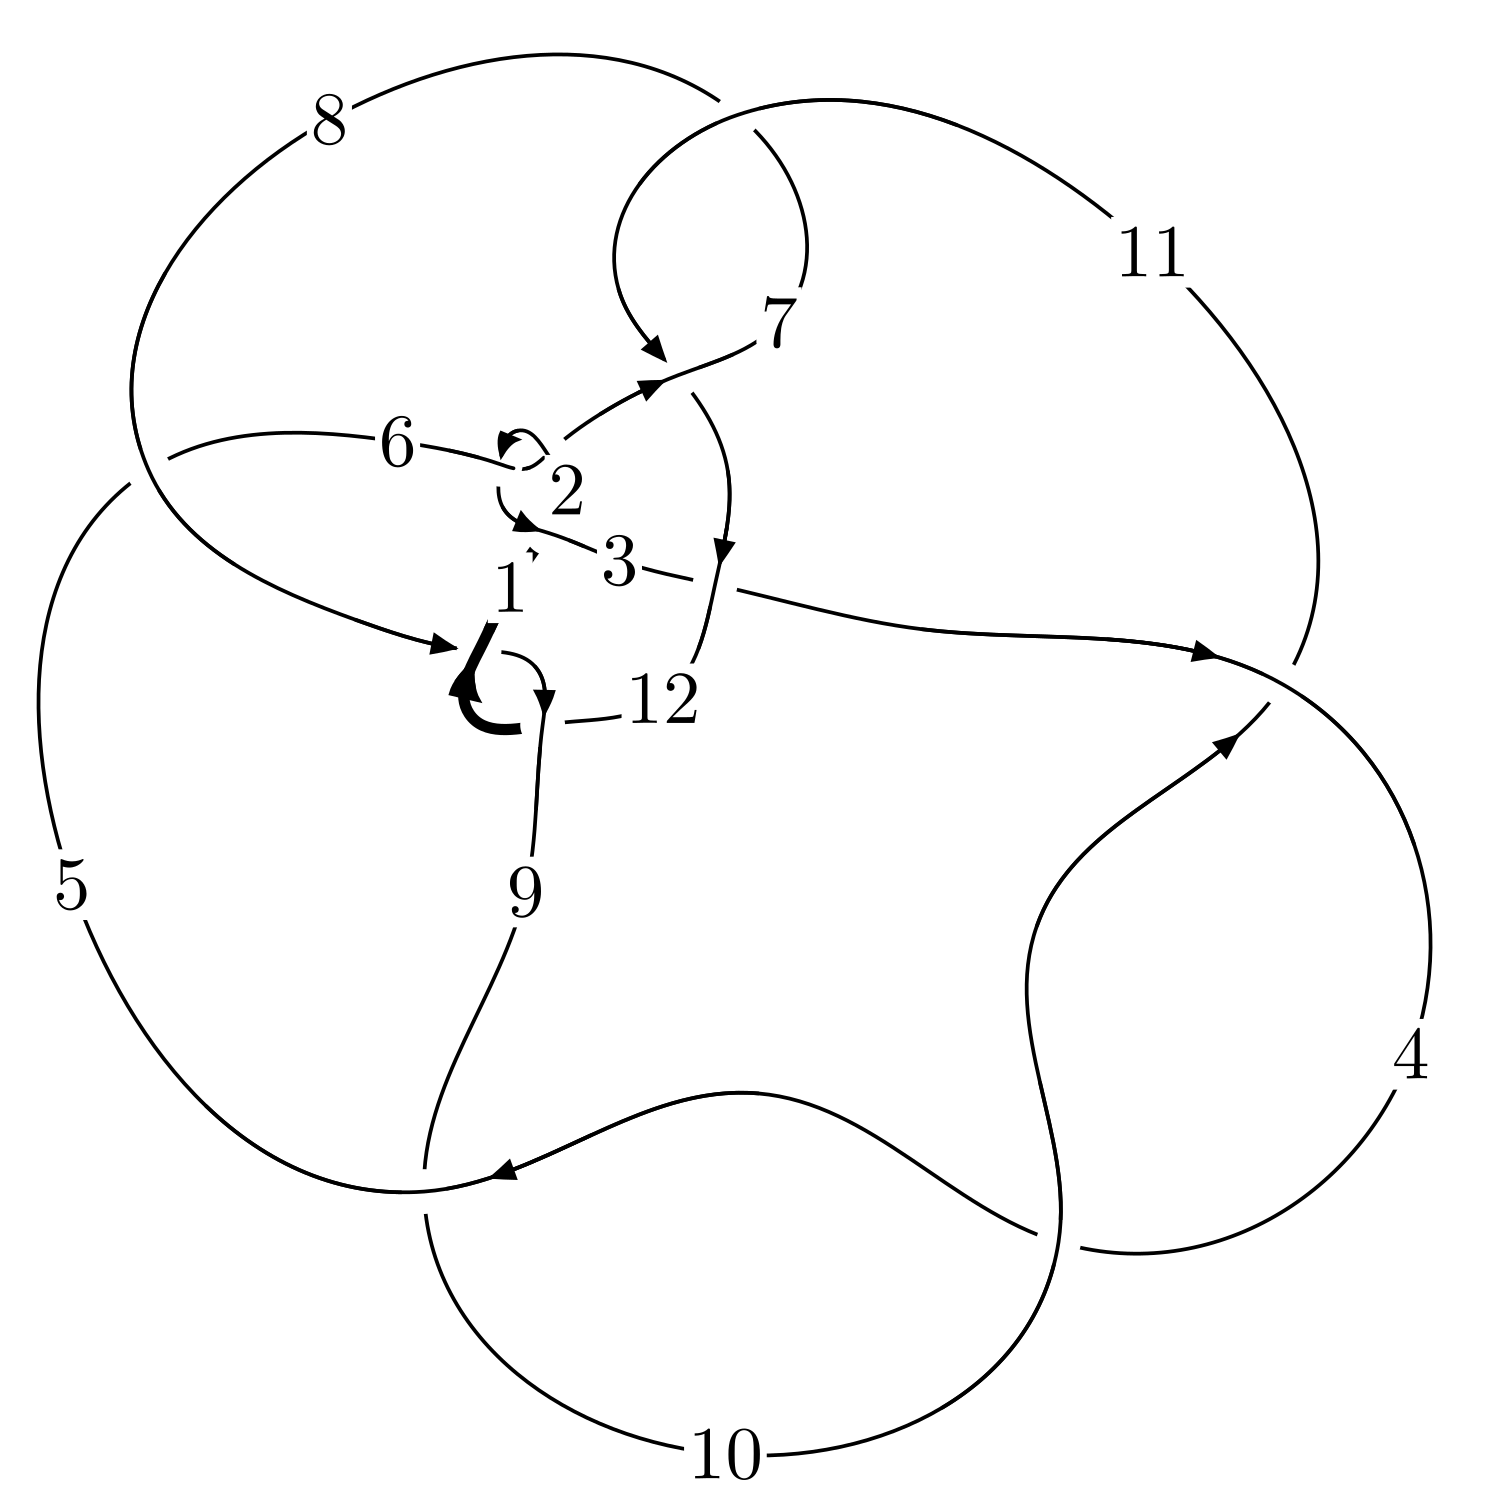
\includegraphics[width=112pt]{../../../GIT/diagram.site/Diagrams/png/1295_12a_0494.png}\\
\ \ \ A knot diagram\footnotemark}&
\allowdisplaybreaks
\textbf{Linearized knot diagam} \\
\cline{2-2}
 &
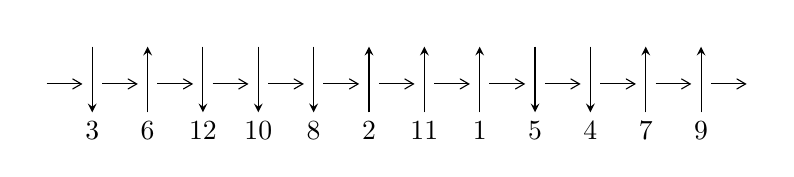
\begin{tikzpicture}[x=20pt, y=17pt]
	% nodes
	\node (C0) at (0, 0) {};
	\node (C1) at (1, 0) {};
	\node (C1U) at (1, +1) {};
	\node (C1D) at (1, -1) {3};

	\node (C2) at (2, 0) {};
	\node (C2U) at (2, +1) {};
	\node (C2D) at (2, -1) {6};

	\node (C3) at (3, 0) {};
	\node (C3U) at (3, +1) {};
	\node (C3D) at (3, -1) {12};

	\node (C4) at (4, 0) {};
	\node (C4U) at (4, +1) {};
	\node (C4D) at (4, -1) {10};

	\node (C5) at (5, 0) {};
	\node (C5U) at (5, +1) {};
	\node (C5D) at (5, -1) {8};

	\node (C6) at (6, 0) {};
	\node (C6U) at (6, +1) {};
	\node (C6D) at (6, -1) {2};

	\node (C7) at (7, 0) {};
	\node (C7U) at (7, +1) {};
	\node (C7D) at (7, -1) {11};

	\node (C8) at (8, 0) {};
	\node (C8U) at (8, +1) {};
	\node (C8D) at (8, -1) {1};

	\node (C9) at (9, 0) {};
	\node (C9U) at (9, +1) {};
	\node (C9D) at (9, -1) {5};

	\node (C10) at (10, 0) {};
	\node (C10U) at (10, +1) {};
	\node (C10D) at (10, -1) {4};

	\node (C11) at (11, 0) {};
	\node (C11U) at (11, +1) {};
	\node (C11D) at (11, -1) {7};

	\node (C12) at (12, 0) {};
	\node (C12U) at (12, +1) {};
	\node (C12D) at (12, -1) {9};
	\node (C13) at (13, 0) {};

	% arrows
	\draw[->,>={angle 60}]
	(C0) edge (C1) (C1) edge (C2) (C2) edge (C3) (C3) edge (C4) (C4) edge (C5) (C5) edge (C6) (C6) edge (C7) (C7) edge (C8) (C8) edge (C9) (C9) edge (C10) (C10) edge (C11) (C11) edge (C12) (C12) edge (C13) ;	\draw[->,>=stealth]
	(C1U) edge (C1D) (C2D) edge (C2U) (C3U) edge (C3D) (C4U) edge (C4D) (C5U) edge (C5D) (C6D) edge (C6U) (C7D) edge (C7U) (C8D) edge (C8U) (C9U) edge (C9D) (C10U) edge (C10D) (C11D) edge (C11U) (C12D) edge (C12U) ;
	\end{tikzpicture} \\
\hhline{~~} \\& 
\textbf{Solving Sequence} \\ \cline{2-2} 
 &
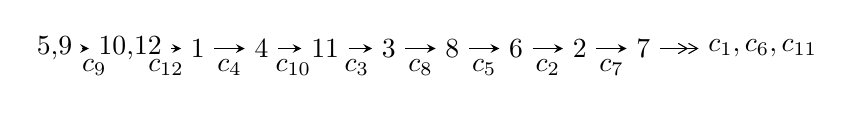
\begin{tikzpicture}[x=23pt, y=7pt]
	% node
	\node (A0) at (-1/8, 0) {5,9};
	\node (A1) at (17/16, 0) {10,12};
	\node (A2) at (17/8, 0) {1};
	\node (A3) at (25/8, 0) {4};
	\node (A4) at (33/8, 0) {11};
	\node (A5) at (41/8, 0) {3};
	\node (A6) at (49/8, 0) {8};
	\node (A7) at (57/8, 0) {6};
	\node (A8) at (65/8, 0) {2};
	\node (A9) at (73/8, 0) {7};
	\node (C1) at (1/2, -1) {$c_{9}$};
	\node (C2) at (13/8, -1) {$c_{12}$};
	\node (C3) at (21/8, -1) {$c_{4}$};
	\node (C4) at (29/8, -1) {$c_{10}$};
	\node (C5) at (37/8, -1) {$c_{3}$};
	\node (C6) at (45/8, -1) {$c_{8}$};
	\node (C7) at (53/8, -1) {$c_{5}$};
	\node (C8) at (61/8, -1) {$c_{2}$};
	\node (C9) at (69/8, -1) {$c_{7}$};
	\node (A10) at (11, 0) {$c_{1},c_{6},c_{11}$};

	% edge
	\draw[->,>=stealth]	
	(A0) edge (A1) (A1) edge (A2) (A2) edge (A3) (A3) edge (A4) (A4) edge (A5) (A5) edge (A6) (A6) edge (A7) (A7) edge (A8) (A8) edge (A9) ;
	\draw[->>,>={angle 60}]	
	(A9) edge (A10);
\end{tikzpicture} \\ 

\end{tabular} \\

\footnotetext{
The image of knot diagram is generated by the software ``\textbf{Draw programme}" developed by Andrew Bartholomew(\url{http://www.layer8.co.uk/maths/draw/index.htm\#Running-draw}), where we modified some parts for our purpose(\url{https://github.com/CATsTAILs/LinksPainter}).
}\phantom \\ \newline 
\centering \textbf{Ideals for irreducible components\footnotemark of $X_{\text{par}}$} 
 
\begin{align*}
I^u_{1}&=\langle 
2.59322\times10^{61} u^{45}-6.46819\times10^{61} u^{44}+\cdots+5.94180\times10^{62} b-7.19573\times10^{62},\\
\phantom{I^u_{1}}&\phantom{= \langle  }-5.17566\times10^{61} u^{45}+1.21957\times10^{62} u^{44}+\cdots+4.75344\times10^{63} a-2.87479\times10^{61},\\
\phantom{I^u_{1}}&\phantom{= \langle  }u^{46}-3 u^{45}+\cdots-224 u+32\rangle \\
I^u_{2}&=\langle 
95 u^{32} a-243 u^{32}+\cdots+483 a-3272,\;30 u^{32} a-55 u^{32}+\cdots+33 a-86,\;u^{33}+u^{32}+\cdots+3 u+1\rangle \\
I^u_{3}&=\langle 
- u^5+b- u,\;u^5-4 u^4- u^3-3 u^2+7 a+4 u-9,\;u^6+u^4+2 u^2+1\rangle \\
I^u_{4}&=\langle 
b-1,\;8 a^2-2 a u+24 a-3 u+17,\;u^2+2\rangle \\
\\
I^v_{1}&=\langle 
a,\;b+1,\;4 v^2-2 v+1\rangle \\
\end{align*}
\raggedright * 5 irreducible components of $\dim_{\mathbb{C}}=0$, with total 124 representations.\\
\footnotetext{All coefficients of polynomials are rational numbers. But the coefficients are sometimes approximated in decimal forms when there is not enough margin.}
\newpage
\renewcommand{\arraystretch}{1}
\centering \section*{I. $I^u_{1}= \langle 2.59\times10^{61} u^{45}-6.47\times10^{61} u^{44}+\cdots+5.94\times10^{62} b-7.20\times10^{62},\;-5.18\times10^{61} u^{45}+1.22\times10^{62} u^{44}+\cdots+4.75\times10^{63} a-2.87\times10^{61},\;u^{46}-3 u^{45}+\cdots-224 u+32 \rangle$}
\flushleft \textbf{(i) Arc colorings}\\
\begin{tabular}{m{7pt} m{180pt} m{7pt} m{180pt} }
\flushright $a_{5}=$&$\begin{pmatrix}0\\u\end{pmatrix}$ \\
\flushright $a_{9}=$&$\begin{pmatrix}1\\0\end{pmatrix}$ \\
\flushright $a_{10}=$&$\begin{pmatrix}1\\u^2\end{pmatrix}$ \\
\flushright $a_{12}=$&$\begin{pmatrix}0.0108883 u^{45}-0.0256565 u^{44}+\cdots+2.71425 u+0.00604782\\-0.0436437 u^{45}+0.108859 u^{44}+\cdots-11.8294 u+1.21104\end{pmatrix}$ \\
\flushright $a_{1}=$&$\begin{pmatrix}-0.0327555 u^{45}+0.0832026 u^{44}+\cdots-9.11514 u+1.21708\\-0.0436437 u^{45}+0.108859 u^{44}+\cdots-11.8294 u+1.21104\end{pmatrix}$ \\
\flushright $a_{4}=$&$\begin{pmatrix}u\\u^3+u\end{pmatrix}$ \\
\flushright $a_{11}=$&$\begin{pmatrix}u^2+1\\u^4+2 u^2\end{pmatrix}$ \\
\flushright $a_{3}=$&$\begin{pmatrix}0.0404758 u^{45}-0.0994274 u^{44}+\cdots+13.5494 u-2.27268\\-0.0314148 u^{45}+0.0849635 u^{44}+\cdots-11.6220 u+2.15240\end{pmatrix}$ \\
\flushright $a_{8}=$&$\begin{pmatrix}0.0566730 u^{45}-0.138814 u^{44}+\cdots+15.7651 u-1.42925\\0.0599305 u^{45}-0.148388 u^{44}+\cdots+18.2271 u-2.43384\end{pmatrix}$ \\
\flushright $a_{6}=$&$\begin{pmatrix}-0.0811578 u^{45}+0.209282 u^{44}+\cdots-28.8041 u+5.12908\\-0.0530046 u^{45}+0.138397 u^{44}+\cdots-20.3166 u+3.95052\end{pmatrix}$ \\
\flushright $a_{2}=$&$\begin{pmatrix}0.0304632 u^{45}-0.0783396 u^{44}+\cdots+13.8672 u-3.59282\\-0.0360975 u^{45}+0.0959193 u^{44}+\cdots-13.5985 u+1.99297\end{pmatrix}$ \\
\flushright $a_{7}=$&$\begin{pmatrix}0.00825991 u^{45}-0.0153222 u^{44}+\cdots+0.388121 u+0.488092\\0.0450341 u^{45}-0.106499 u^{44}+\cdots+11.3574 u-1.03163\end{pmatrix}$\\&\end{tabular}
\flushleft \textbf{(ii) Obstruction class $= -1$}\\~\\
\flushleft \textbf{(iii) Cusp Shapes $= 0.447426 u^{45}-1.30981 u^{44}+\cdots+236.624 u-56.0043$}\\~\\
\newpage\renewcommand{\arraystretch}{1}
\flushleft \textbf{(iv) u-Polynomials at the component}\newline \\
\begin{tabular}{m{50pt}|m{274pt}}
Crossings & \hspace{64pt}u-Polynomials at each crossing \\
\hline $$\begin{aligned}c_{1}\end{aligned}$$&$\begin{aligned}
&u^{46}+24 u^{45}+\cdots+1295 u+576
\end{aligned}$\\
\hline $$\begin{aligned}c_{2},c_{6}\end{aligned}$$&$\begin{aligned}
&u^{46}-2 u^{45}+\cdots-71 u+24
\end{aligned}$\\
\hline $$\begin{aligned}c_{3},c_{5}\end{aligned}$$&$\begin{aligned}
&64(64 u^{46}-160 u^{45}+\cdots+146 u+11)
\end{aligned}$\\
\hline $$\begin{aligned}c_{4},c_{9},c_{10}\end{aligned}$$&$\begin{aligned}
&u^{46}+3 u^{45}+\cdots+224 u+32
\end{aligned}$\\
\hline $$\begin{aligned}c_{7},c_{8},c_{11}\\c_{12}\end{aligned}$$&$\begin{aligned}
&u^{46}+2 u^{45}+\cdots+8 u+3
\end{aligned}$\\
\hline
\end{tabular}\\~\\
\newpage\renewcommand{\arraystretch}{1}
\flushleft \textbf{(v) Riley Polynomials at the component}\newline \\
\begin{tabular}{m{50pt}|m{274pt}}
Crossings & \hspace{64pt}Riley Polynomials at each crossing \\
\hline $$\begin{aligned}c_{1}\end{aligned}$$&$\begin{aligned}
&y^{46}+16 y^{44}+\cdots+13494815 y+331776
\end{aligned}$\\
\hline $$\begin{aligned}c_{2},c_{6}\end{aligned}$$&$\begin{aligned}
&y^{46}+24 y^{45}+\cdots+1295 y+576
\end{aligned}$\\
\hline $$\begin{aligned}c_{3},c_{5}\end{aligned}$$&$\begin{aligned}
&4096(4096 y^{46}+60416 y^{45}+\cdots+3104 y+121)
\end{aligned}$\\
\hline $$\begin{aligned}c_{4},c_{9},c_{10}\end{aligned}$$&$\begin{aligned}
&y^{46}+41 y^{45}+\cdots-5120 y+1024
\end{aligned}$\\
\hline $$\begin{aligned}c_{7},c_{8},c_{11}\\c_{12}\end{aligned}$$&$\begin{aligned}
&y^{46}+14 y^{45}+\cdots+302 y+9
\end{aligned}$\\
\hline
\end{tabular}\\~\\
\newpage\flushleft \textbf{(vi) Complex Volumes and Cusp Shapes}
$$\begin{array}{c|c|c}  
\text{Solutions to }I^u_{1}& \I (\text{vol} + \sqrt{-1}CS) & \text{Cusp shape}\\
 \hline 
\begin{aligned}
u &= \phantom{-}0.879927 + 0.422250 I \\
a &= -1.002480 - 0.651826 I \\
b &= \phantom{-}0.561540 - 1.266480 I\end{aligned}
 & -5.3080 - 13.9989 I & -4.18038 + 9.68220 I \\ \hline\begin{aligned}
u &= \phantom{-}0.879927 - 0.422250 I \\
a &= -1.002480 + 0.651826 I \\
b &= \phantom{-}0.561540 + 1.266480 I\end{aligned}
 & -5.3080 + 13.9989 I & -4.18038 - 9.68220 I \\ \hline\begin{aligned}
u &= -0.884396 + 0.372933 I \\
a &= -0.864488 + 0.759473 I \\
b &= \phantom{-}0.533136 + 1.175940 I\end{aligned}
 & -2.75455 + 8.29717 I & -1.70737 - 6.58630 I \\ \hline\begin{aligned}
u &= -0.884396 - 0.372933 I \\
a &= -0.864488 - 0.759473 I \\
b &= \phantom{-}0.533136 - 1.175940 I\end{aligned}
 & -2.75455 - 8.29717 I & -1.70737 + 6.58630 I \\ \hline\begin{aligned}
u &= \phantom{-}1.005690 + 0.347417 I \\
a &= -0.592795 - 0.569917 I \\
b &= \phantom{-}0.354628 - 1.155160 I\end{aligned}
 & -8.53774 - 4.63661 I & -7.26779 + 6.24429 I \\ \hline\begin{aligned}
u &= \phantom{-}1.005690 - 0.347417 I \\
a &= -0.592795 + 0.569917 I \\
b &= \phantom{-}0.354628 + 1.155160 I\end{aligned}
 & -8.53774 + 4.63661 I & -7.26779 - 6.24429 I \\ \hline\begin{aligned}
u &= \phantom{-}0.757476 + 0.798859 I \\
a &= -0.138023 + 0.165827 I \\
b &= -0.458745 - 1.156100 I\end{aligned}
 & -4.22061 + 8.47102 I & -3.55506 - 6.39259 I \\ \hline\begin{aligned}
u &= \phantom{-}0.757476 - 0.798859 I \\
a &= -0.138023 - 0.165827 I \\
b &= -0.458745 + 1.156100 I\end{aligned}
 & -4.22061 - 8.47102 I & -3.55506 + 6.39259 I \\ \hline\begin{aligned}
u &= -0.677203 + 0.890151 I \\
a &= -0.1047750 - 0.0770628 I \\
b &= -0.426999 + 1.020500 I\end{aligned}
 & -1.24313 - 2.90152 I & \phantom{-0.000000 -}0. + 4.04088 I \\ \hline\begin{aligned}
u &= -0.677203 - 0.890151 I \\
a &= -0.1047750 + 0.0770628 I \\
b &= -0.426999 - 1.020500 I\end{aligned}
 & -1.24313 + 2.90152 I & \phantom{-0.000000 } 0. - 4.04088 I\\
 \hline 
 \end{array}$$\newpage$$\begin{array}{c|c|c}  
\text{Solutions to }I^u_{1}& \I (\text{vol} + \sqrt{-1}CS) & \text{Cusp shape}\\
 \hline 
\begin{aligned}
u &= -0.754848 + 0.065218 I \\
a &= -0.005515 + 1.244420 I \\
b &= \phantom{-}0.435207 + 0.754548 I\end{aligned}
 & \phantom{-}0.39391 + 4.28987 I & -0.46705 - 7.97221 I \\ \hline\begin{aligned}
u &= -0.754848 - 0.065218 I \\
a &= -0.005515 - 1.244420 I \\
b &= \phantom{-}0.435207 - 0.754548 I\end{aligned}
 & \phantom{-}0.39391 - 4.28987 I & -0.46705 + 7.97221 I \\ \hline\begin{aligned}
u &= -0.899443 + 0.871931 I \\
a &= \phantom{-}0.417382 - 0.332407 I \\
b &= -0.087635 - 0.831168 I\end{aligned}
 & -5.56613 + 3.24368 I & \phantom{-0.000000 } 0 \\ \hline\begin{aligned}
u &= -0.899443 - 0.871931 I \\
a &= \phantom{-}0.417382 + 0.332407 I \\
b &= -0.087635 + 0.831168 I\end{aligned}
 & -5.56613 - 3.24368 I & \phantom{-0.000000 } 0 \\ \hline\begin{aligned}
u &= \phantom{-}0.053471 + 1.326470 I \\
a &= -2.00960 - 0.27769 I \\
b &= \phantom{-}1.397470 + 0.175373 I\end{aligned}
 & \phantom{-}5.26321 + 1.38773 I & \phantom{-0.000000 } 0 \\ \hline\begin{aligned}
u &= \phantom{-}0.053471 - 1.326470 I \\
a &= -2.00960 + 0.27769 I \\
b &= \phantom{-}1.397470 - 0.175373 I\end{aligned}
 & \phantom{-}5.26321 - 1.38773 I & \phantom{-0.000000 } 0 \\ \hline\begin{aligned}
u &= \phantom{-}0.348272 + 1.303000 I \\
a &= \phantom{-}1.089410 + 0.524655 I \\
b &= -0.515748 + 0.904481 I\end{aligned}
 & \phantom{-}4.21026 - 2.45289 I & \phantom{-0.000000 } 0 \\ \hline\begin{aligned}
u &= \phantom{-}0.348272 - 1.303000 I \\
a &= \phantom{-}1.089410 - 0.524655 I \\
b &= -0.515748 - 0.904481 I\end{aligned}
 & \phantom{-}4.21026 + 2.45289 I & \phantom{-0.000000 } 0 \\ \hline\begin{aligned}
u &= \phantom{-}0.785322 + 1.112070 I \\
a &= -0.189157 + 0.017429 I \\
b &= -0.244145 - 0.990574 I\end{aligned}
 & -6.40579 - 1.59325 I & \phantom{-0.000000 } 0 \\ \hline\begin{aligned}
u &= \phantom{-}0.785322 - 1.112070 I \\
a &= -0.189157 - 0.017429 I \\
b &= -0.244145 + 0.990574 I\end{aligned}
 & -6.40579 + 1.59325 I & \phantom{-0.000000 } 0\\
 \hline 
 \end{array}$$\newpage$$\begin{array}{c|c|c}  
\text{Solutions to }I^u_{1}& \I (\text{vol} + \sqrt{-1}CS) & \text{Cusp shape}\\
 \hline 
\begin{aligned}
u &= \phantom{-}0.146892 + 1.387240 I \\
a &= -1.75835 - 0.81715 I \\
b &= \phantom{-}1.34196 + 0.58047 I\end{aligned}
 & \phantom{-}6.66740 - 4.38324 I & \phantom{-0.000000 } 0 \\ \hline\begin{aligned}
u &= \phantom{-}0.146892 - 1.387240 I \\
a &= -1.75835 + 0.81715 I \\
b &= \phantom{-}1.34196 - 0.58047 I\end{aligned}
 & \phantom{-}6.66740 + 4.38324 I & \phantom{-0.000000 } 0 \\ \hline\begin{aligned}
u &= -0.34923 + 1.38244 I \\
a &= \phantom{-}1.349640 - 0.348220 I \\
b &= -0.570864 - 1.015940 I\end{aligned}
 & \phantom{-}5.05332 + 8.42012 I & \phantom{-0.000000 } 0 \\ \hline\begin{aligned}
u &= -0.34923 - 1.38244 I \\
a &= \phantom{-}1.349640 + 0.348220 I \\
b &= -0.570864 + 1.015940 I\end{aligned}
 & \phantom{-}5.05332 - 8.42012 I & \phantom{-0.000000 } 0 \\ \hline\begin{aligned}
u &= -0.12544 + 1.43283 I \\
a &= -1.49007 + 0.74151 I \\
b &= \phantom{-}1.133480 - 0.604428 I\end{aligned}
 & \phantom{-}8.14786 - 0.11264 I & \phantom{-0.000000 } 0 \\ \hline\begin{aligned}
u &= -0.12544 - 1.43283 I \\
a &= -1.49007 - 0.74151 I \\
b &= \phantom{-}1.133480 + 0.604428 I\end{aligned}
 & \phantom{-}8.14786 + 0.11264 I & \phantom{-0.000000 } 0 \\ \hline\begin{aligned}
u &= \phantom{-}0.545297 + 0.078664 I \\
a &= \phantom{-}0.83525 + 1.15694 I \\
b &= \phantom{-}0.339032 + 0.466799 I\end{aligned}
 & \phantom{-}0.445010 - 1.185620 I & -1.75729 - 0.29982 I \\ \hline\begin{aligned}
u &= \phantom{-}0.545297 - 0.078664 I \\
a &= \phantom{-}0.83525 - 1.15694 I \\
b &= \phantom{-}0.339032 - 0.466799 I\end{aligned}
 & \phantom{-}0.445010 + 1.185620 I & -1.75729 + 0.29982 I \\ \hline\begin{aligned}
u &= -0.05409 + 1.45463 I \\
a &= -0.840100 - 0.001476 I \\
b &= \phantom{-}0.128963 + 0.320779 I\end{aligned}
 & \phantom{-}4.81424 - 1.83892 I & \phantom{-0.000000 } 0 \\ \hline\begin{aligned}
u &= -0.05409 - 1.45463 I \\
a &= -0.840100 + 0.001476 I \\
b &= \phantom{-}0.128963 - 0.320779 I\end{aligned}
 & \phantom{-}4.81424 + 1.83892 I & \phantom{-0.000000 } 0\\
 \hline 
 \end{array}$$\newpage$$\begin{array}{c|c|c}  
\text{Solutions to }I^u_{1}& \I (\text{vol} + \sqrt{-1}CS) & \text{Cusp shape}\\
 \hline 
\begin{aligned}
u &= \phantom{-}0.271343 + 0.437430 I \\
a &= \phantom{-}0.674777 + 0.345785 I \\
b &= -0.143974 + 0.371385 I\end{aligned}
 & \phantom{-}0.079000 - 0.909335 I & \phantom{-}2.05664 + 7.20006 I \\ \hline\begin{aligned}
u &= \phantom{-}0.271343 - 0.437430 I \\
a &= \phantom{-}0.674777 - 0.345785 I \\
b &= -0.143974 - 0.371385 I\end{aligned}
 & \phantom{-}0.079000 + 0.909335 I & \phantom{-}2.05664 - 7.20006 I \\ \hline\begin{aligned}
u &= -0.287009 + 0.385178 I \\
a &= \phantom{-}0.422708 - 0.041305 I \\
b &= -0.918597 + 0.410101 I\end{aligned}
 & \phantom{-}2.29870 - 1.77899 I & \phantom{-}6.01313 - 3.03294 I \\ \hline\begin{aligned}
u &= -0.287009 - 0.385178 I \\
a &= \phantom{-}0.422708 + 0.041305 I \\
b &= -0.918597 - 0.410101 I\end{aligned}
 & \phantom{-}2.29870 + 1.77899 I & \phantom{-}6.01313 + 3.03294 I \\ \hline\begin{aligned}
u &= -0.33737 + 1.48238 I \\
a &= \phantom{-}1.70844 + 0.12166 I \\
b &= -0.646202 - 1.244350 I\end{aligned}
 & \phantom{-}3.20888 + 12.70970 I & \phantom{-0.000000 } 0 \\ \hline\begin{aligned}
u &= -0.33737 - 1.48238 I \\
a &= \phantom{-}1.70844 - 0.12166 I \\
b &= -0.646202 + 1.244350 I\end{aligned}
 & \phantom{-}3.20888 - 12.70970 I & \phantom{-0.000000 } 0 \\ \hline\begin{aligned}
u &= -0.06899 + 1.52703 I \\
a &= -0.969248 + 0.549033 I \\
b &= \phantom{-}0.669287 - 0.651303 I\end{aligned}
 & \phantom{-}7.27063 - 1.16863 I & \phantom{-0.000000 } 0 \\ \hline\begin{aligned}
u &= -0.06899 - 1.52703 I \\
a &= -0.969248 - 0.549033 I \\
b &= \phantom{-}0.669287 + 0.651303 I\end{aligned}
 & \phantom{-}7.27063 + 1.16863 I & \phantom{-0.000000 } 0 \\ \hline\begin{aligned}
u &= \phantom{-}0.38401 + 1.48415 I \\
a &= \phantom{-}1.41083 - 0.19362 I \\
b &= -0.513706 + 1.238240 I\end{aligned}
 & -2.67740 - 9.58899 I & \phantom{-0.000000 } 0 \\ \hline\begin{aligned}
u &= \phantom{-}0.38401 - 1.48415 I \\
a &= \phantom{-}1.41083 + 0.19362 I \\
b &= -0.513706 - 1.238240 I\end{aligned}
 & -2.67740 + 9.58899 I & \phantom{-0.000000 } 0\\
 \hline 
 \end{array}$$\newpage$$\begin{array}{c|c|c}  
\text{Solutions to }I^u_{1}& \I (\text{vol} + \sqrt{-1}CS) & \text{Cusp shape}\\
 \hline 
\begin{aligned}
u &= \phantom{-}0.33179 + 1.50033 I \\
a &= \phantom{-}1.78862 - 0.24742 I \\
b &= -0.66692 + 1.30465 I\end{aligned}
 & \phantom{-}0.8798 - 18.3922 I & \phantom{-0.000000 } 0 \\ \hline\begin{aligned}
u &= \phantom{-}0.33179 - 1.50033 I \\
a &= \phantom{-}1.78862 + 0.24742 I \\
b &= -0.66692 - 1.30465 I\end{aligned}
 & \phantom{-}0.8798 + 18.3922 I & \phantom{-0.000000 } 0 \\ \hline\begin{aligned}
u &= \phantom{-}0.349735 + 0.181130 I \\
a &= \phantom{-}0.516188 + 0.059087 I \\
b &= -1.173810 - 0.239503 I\end{aligned}
 & \phantom{-}1.57408 - 2.45072 I & -5.4120 + 13.0814 I \\ \hline\begin{aligned}
u &= \phantom{-}0.349735 - 0.181130 I \\
a &= \phantom{-}0.516188 - 0.059087 I \\
b &= -1.173810 + 0.239503 I\end{aligned}
 & \phantom{-}1.57408 + 2.45072 I & -5.4120 - 13.0814 I \\ \hline\begin{aligned}
u &= \phantom{-}0.07879 + 1.62688 I \\
a &= -0.623636 - 0.621149 I \\
b &= \phantom{-}0.472651 + 0.872181 I\end{aligned}
 & \phantom{-}4.50126 + 5.50730 I & \phantom{-0.000000 } 0 \\ \hline\begin{aligned}
u &= \phantom{-}0.07879 - 1.62688 I \\
a &= -0.623636 + 0.621149 I \\
b &= \phantom{-}0.472651 - 0.872181 I\end{aligned}
 & \phantom{-}4.50126 - 5.50730 I & \phantom{-0.000000 } 0\\
 \hline 
 \end{array}$$\newpage\newpage\renewcommand{\arraystretch}{1}
\centering \section*{II. $I^u_{2}= \langle 95 u^{32} a-243 u^{32}+\cdots+483 a-3272,\;30 u^{32} a-55 u^{32}+\cdots+33 a-86,\;u^{33}+u^{32}+\cdots+3 u+1 \rangle$}
\flushleft \textbf{(i) Arc colorings}\\
\begin{tabular}{m{7pt} m{180pt} m{7pt} m{180pt} }
\flushright $a_{5}=$&$\begin{pmatrix}0\\u\end{pmatrix}$ \\
\flushright $a_{9}=$&$\begin{pmatrix}1\\0\end{pmatrix}$ \\
\flushright $a_{10}=$&$\begin{pmatrix}1\\u^2\end{pmatrix}$ \\
\flushright $a_{12}=$&$\begin{pmatrix}a\\-0.0387913 a u^{32}+0.0992242 u^{32}+\cdots-0.197223 a+1.33606\end{pmatrix}$ \\
\flushright $a_{1}=$&$\begin{pmatrix}-0.0387913 a u^{32}+0.0992242 u^{32}+\cdots+0.802777 a+1.33606\\-0.0387913 a u^{32}+0.0992242 u^{32}+\cdots-0.197223 a+1.33606\end{pmatrix}$ \\
\flushright $a_{4}=$&$\begin{pmatrix}u\\u^3+u\end{pmatrix}$ \\
\flushright $a_{11}=$&$\begin{pmatrix}u^2+1\\u^4+2 u^2\end{pmatrix}$ \\
\flushright $a_{3}=$&$\begin{pmatrix}1.86661 a u^{32}-0.313779 u^{32}+\cdots+2.56744 a-3.08421\\0.138832 a u^{32}+0.469443 u^{32}+\cdots+0.0216415 a+3.39377\end{pmatrix}$ \\
\flushright $a_{8}=$&$\begin{pmatrix}-0.0387913 a u^{32}-2.56744 u^{32}+\cdots-1.19722 a-2.99728\\0.0604328 a u^{32}-0.0387913 u^{32}+\cdots+0.138832 a-1.19722\end{pmatrix}$ \\
\flushright $a_{6}=$&$\begin{pmatrix}0.191779 a u^{32}+2.84161 u^{32}+\cdots+3.35048 a-3.60410\\-0.277664 a u^{32}+1.72778 u^{32}+\cdots-0.0432830 a+2.54580\end{pmatrix}$ \\
\flushright $a_{2}=$&$\begin{pmatrix}0.748741 a u^{32}-1.53391 u^{32}+\cdots+2.41377 a+0.163831\\-0.246223 a u^{32}-0.731591 u^{32}+\cdots-0.241323 a+1.84184\end{pmatrix}$ \\
\flushright $a_{7}=$&$\begin{pmatrix}-0.0992242 a u^{32}-2.52865 u^{32}+\cdots-1.33606 a-3.80005\\-1\end{pmatrix}$\\&\end{tabular}
\flushleft \textbf{(ii) Obstruction class $= -1$}\\~\\
\flushleft \textbf{(iii) Cusp Shapes $= -4 u^{32}-4 u^{31}-64 u^{30}-56 u^{29}-448 u^{28}-340 u^{27}-1788 u^{26}-1156 u^{25}-4432 u^{24}-2356 u^{23}-6940 u^{22}-2804 u^{21}-6652 u^{20}-1616 u^{19}-3660 u^{18}-8 u^{17}-1380 u^{16}+364 u^{15}-932 u^{14}+156 u^{13}-380 u^{12}+360 u^{11}+224 u^{10}+328 u^9+40 u^8+4 u^7-56 u^6-4 u^5+48 u^4+32 u^3-12 u^2-20 u-10$}\\~\\
\newpage\renewcommand{\arraystretch}{1}
\flushleft \textbf{(iv) u-Polynomials at the component}\newline \\
\begin{tabular}{m{50pt}|m{274pt}}
Crossings & \hspace{64pt}u-Polynomials at each crossing \\
\hline $$\begin{aligned}c_{1}\end{aligned}$$&$\begin{aligned}
&(u^{33}+15 u^{32}+\cdots+u-1)^{2}
\end{aligned}$\\
\hline $$\begin{aligned}c_{2},c_{6}\end{aligned}$$&$\begin{aligned}
&(u^{33}- u^{32}+\cdots- u+1)^{2}
\end{aligned}$\\
\hline $$\begin{aligned}c_{3},c_{5}\end{aligned}$$&$\begin{aligned}
&9(9 u^{66}+129 u^{65}+\cdots+233684 u+29567)
\end{aligned}$\\
\hline $$\begin{aligned}c_{4},c_{9},c_{10}\end{aligned}$$&$\begin{aligned}
&(u^{33}- u^{32}+\cdots+3 u-1)^{2}
\end{aligned}$\\
\hline $$\begin{aligned}c_{7},c_{8},c_{11}\\c_{12}\end{aligned}$$&$\begin{aligned}
&u^{66}-5 u^{65}+\cdots-804 u+125
\end{aligned}$\\
\hline
\end{tabular}\\~\\
\newpage\renewcommand{\arraystretch}{1}
\flushleft \textbf{(v) Riley Polynomials at the component}\newline \\
\begin{tabular}{m{50pt}|m{274pt}}
Crossings & \hspace{64pt}Riley Polynomials at each crossing \\
\hline $$\begin{aligned}c_{1}\end{aligned}$$&$\begin{aligned}
&(y^{33}+7 y^{32}+\cdots+17 y-1)^{2}
\end{aligned}$\\
\hline $$\begin{aligned}c_{2},c_{6}\end{aligned}$$&$\begin{aligned}
&(y^{33}+15 y^{32}+\cdots+y-1)^{2}
\end{aligned}$\\
\hline $$\begin{aligned}c_{3},c_{5}\end{aligned}$$&$\begin{aligned}
&81(81 y^{66}-1701 y^{65}+\cdots-4.02404\times10^{10} y+8.74207\times10^{8})
\end{aligned}$\\
\hline $$\begin{aligned}c_{4},c_{9},c_{10}\end{aligned}$$&$\begin{aligned}
&(y^{33}+31 y^{32}+\cdots+y-1)^{2}
\end{aligned}$\\
\hline $$\begin{aligned}c_{7},c_{8},c_{11}\\c_{12}\end{aligned}$$&$\begin{aligned}
&y^{66}+39 y^{65}+\cdots+129584 y+15625
\end{aligned}$\\
\hline
\end{tabular}\\~\\
\newpage\flushleft \textbf{(vi) Complex Volumes and Cusp Shapes}
$$\begin{array}{c|c|c}  
\text{Solutions to }I^u_{2}& \I (\text{vol} + \sqrt{-1}CS) & \text{Cusp shape}\\
 \hline 
\begin{aligned}
u &= \phantom{-}0.138722 + 1.178260 I \\
a &= \phantom{-}0.646725 + 0.922454 I \\
b &= -0.34986 - 1.41730 I\end{aligned}
 & -3.68002 + 0.57246 I & -4.31906 - 0.48605 I \\ \hline\begin{aligned}
u &= \phantom{-}0.138722 + 1.178260 I \\
a &= \phantom{-}1.89541 - 0.83665 I \\
b &= -0.620802 + 1.176010 I\end{aligned}
 & -3.68002 + 0.57246 I & -4.31906 - 0.48605 I \\ \hline\begin{aligned}
u &= \phantom{-}0.138722 - 1.178260 I \\
a &= \phantom{-}0.646725 - 0.922454 I \\
b &= -0.34986 + 1.41730 I\end{aligned}
 & -3.68002 - 0.57246 I & -4.31906 + 0.48605 I \\ \hline\begin{aligned}
u &= \phantom{-}0.138722 - 1.178260 I \\
a &= \phantom{-}1.89541 + 0.83665 I \\
b &= -0.620802 - 1.176010 I\end{aligned}
 & -3.68002 - 0.57246 I & -4.31906 + 0.48605 I \\ \hline\begin{aligned}
u &= -0.679432 + 0.391507 I \\
a &= \phantom{-}0.967832 - 0.605627 I \\
b &= -0.580882 - 1.258950 I\end{aligned}
 & -1.82082 + 8.41845 I & -1.65597 - 8.08731 I \\ \hline\begin{aligned}
u &= -0.679432 + 0.391507 I \\
a &= -0.492379 + 0.153513 I \\
b &= \phantom{-}1.009630 - 0.133152 I\end{aligned}
 & -1.82082 + 8.41845 I & -1.65597 - 8.08731 I \\ \hline\begin{aligned}
u &= -0.679432 - 0.391507 I \\
a &= \phantom{-}0.967832 + 0.605627 I \\
b &= -0.580882 + 1.258950 I\end{aligned}
 & -1.82082 - 8.41845 I & -1.65597 + 8.08731 I \\ \hline\begin{aligned}
u &= -0.679432 - 0.391507 I \\
a &= -0.492379 - 0.153513 I \\
b &= \phantom{-}1.009630 + 0.133152 I\end{aligned}
 & -1.82082 - 8.41845 I & -1.65597 + 8.08731 I \\ \hline\begin{aligned}
u &= \phantom{-}0.649750 + 0.407780 I \\
a &= \phantom{-}0.961232 + 0.680322 I \\
b &= -0.526453 + 1.104150 I\end{aligned}
 & \phantom{-}0.09121 - 3.30675 I & \phantom{-}1.55576 + 3.71770 I \\ \hline\begin{aligned}
u &= \phantom{-}0.649750 + 0.407780 I \\
a &= -0.320653 - 0.049837 I \\
b &= \phantom{-}0.822908 + 0.226871 I\end{aligned}
 & \phantom{-}0.09121 - 3.30675 I & \phantom{-}1.55576 + 3.71770 I\\
 \hline 
 \end{array}$$\newpage$$\begin{array}{c|c|c}  
\text{Solutions to }I^u_{2}& \I (\text{vol} + \sqrt{-1}CS) & \text{Cusp shape}\\
 \hline 
\begin{aligned}
u &= \phantom{-}0.649750 - 0.407780 I \\
a &= \phantom{-}0.961232 - 0.680322 I \\
b &= -0.526453 - 1.104150 I\end{aligned}
 & \phantom{-}0.09121 + 3.30675 I & \phantom{-}1.55576 - 3.71770 I \\ \hline\begin{aligned}
u &= \phantom{-}0.649750 - 0.407780 I \\
a &= -0.320653 + 0.049837 I \\
b &= \phantom{-}0.822908 - 0.226871 I\end{aligned}
 & \phantom{-}0.09121 + 3.30675 I & \phantom{-}1.55576 - 3.71770 I \\ \hline\begin{aligned}
u &= -0.552937 + 0.519363 I \\
a &= \phantom{-}0.910395 + 0.295741 I \\
b &= \phantom{-}0.356991 - 1.066940 I\end{aligned}
 & -1.29130 - 4.30723 I & -0.15179 + 2.03529 I \\ \hline\begin{aligned}
u &= -0.552937 + 0.519363 I \\
a &= \phantom{-}0.72843 - 1.28598 I \\
b &= -0.613572 - 0.123118 I\end{aligned}
 & -1.29130 - 4.30723 I & -0.15179 + 2.03529 I \\ \hline\begin{aligned}
u &= -0.552937 - 0.519363 I \\
a &= \phantom{-}0.910395 - 0.295741 I \\
b &= \phantom{-}0.356991 + 1.066940 I\end{aligned}
 & -1.29130 + 4.30723 I & -0.15179 - 2.03529 I \\ \hline\begin{aligned}
u &= -0.552937 - 0.519363 I \\
a &= \phantom{-}0.72843 + 1.28598 I \\
b &= -0.613572 + 0.123118 I\end{aligned}
 & -1.29130 + 4.30723 I & -0.15179 - 2.03529 I \\ \hline\begin{aligned}
u &= \phantom{-}0.578988 + 0.474023 I \\
a &= \phantom{-}0.703739 + 0.930950 I \\
b &= -0.406968 + 0.442807 I\end{aligned}
 & \phantom{-}0.382723 - 0.728314 I & \phantom{-}2.50985 + 3.12560 I \\ \hline\begin{aligned}
u &= \phantom{-}0.578988 + 0.474023 I \\
a &= \phantom{-}0.566060 + 0.034191 I \\
b &= \phantom{-}0.338945 + 0.776348 I\end{aligned}
 & \phantom{-}0.382723 - 0.728314 I & \phantom{-}2.50985 + 3.12560 I \\ \hline\begin{aligned}
u &= \phantom{-}0.578988 - 0.474023 I \\
a &= \phantom{-}0.703739 - 0.930950 I \\
b &= -0.406968 - 0.442807 I\end{aligned}
 & \phantom{-}0.382723 + 0.728314 I & \phantom{-}2.50985 - 3.12560 I \\ \hline\begin{aligned}
u &= \phantom{-}0.578988 - 0.474023 I \\
a &= \phantom{-}0.566060 - 0.034191 I \\
b &= \phantom{-}0.338945 - 0.776348 I\end{aligned}
 & \phantom{-}0.382723 + 0.728314 I & \phantom{-}2.50985 - 3.12560 I\\
 \hline 
 \end{array}$$\newpage$$\begin{array}{c|c|c}  
\text{Solutions to }I^u_{2}& \I (\text{vol} + \sqrt{-1}CS) & \text{Cusp shape}\\
 \hline 
\begin{aligned}
u &= \phantom{-}0.214004 + 1.270020 I \\
a &= -0.191089 + 0.920763 I \\
b &= -0.12595 - 1.55585 I\end{aligned}
 & -2.78381 - 6.56196 I & -2.35976 + 7.19745 I \\ \hline\begin{aligned}
u &= \phantom{-}0.214004 + 1.270020 I \\
a &= \phantom{-}2.06381 - 0.68885 I \\
b &= -0.847874 + 0.939274 I\end{aligned}
 & -2.78381 - 6.56196 I & -2.35976 + 7.19745 I \\ \hline\begin{aligned}
u &= \phantom{-}0.214004 - 1.270020 I \\
a &= -0.191089 - 0.920763 I \\
b &= -0.12595 + 1.55585 I\end{aligned}
 & -2.78381 + 6.56196 I & -2.35976 - 7.19745 I \\ \hline\begin{aligned}
u &= \phantom{-}0.214004 - 1.270020 I \\
a &= \phantom{-}2.06381 + 0.68885 I \\
b &= -0.847874 - 0.939274 I\end{aligned}
 & -2.78381 + 6.56196 I & -2.35976 - 7.19745 I \\ \hline\begin{aligned}
u &= -0.150986 + 1.283520 I \\
a &= \phantom{-}0.004911 - 0.404260 I \\
b &= -0.139375 + 1.388990 I\end{aligned}
 & -0.32048 + 2.39560 I & \phantom{-}1.63078 - 3.31266 I \\ \hline\begin{aligned}
u &= -0.150986 + 1.283520 I \\
a &= \phantom{-}2.00230 + 0.72485 I \\
b &= -0.620697 - 0.904803 I\end{aligned}
 & -0.32048 + 2.39560 I & \phantom{-}1.63078 - 3.31266 I \\ \hline\begin{aligned}
u &= -0.150986 - 1.283520 I \\
a &= \phantom{-}0.004911 + 0.404260 I \\
b &= -0.139375 - 1.388990 I\end{aligned}
 & -0.32048 - 2.39560 I & \phantom{-}1.63078 + 3.31266 I \\ \hline\begin{aligned}
u &= -0.150986 - 1.283520 I \\
a &= \phantom{-}2.00230 - 0.72485 I \\
b &= -0.620697 + 0.904803 I\end{aligned}
 & -0.32048 - 2.39560 I & \phantom{-}1.63078 + 3.31266 I \\ \hline\begin{aligned}
u &= -0.596688 + 0.315979 I \\
a &= -0.801138 - 0.348679 I \\
b &= \phantom{-}0.610189 + 0.315745 I\end{aligned}
 & -4.72027 + 1.50384 I & -5.59059 - 3.60616 I \\ \hline\begin{aligned}
u &= -0.596688 + 0.315979 I \\
a &= \phantom{-}0.819943 - 0.823377 I \\
b &= -0.174356 - 1.263120 I\end{aligned}
 & -4.72027 + 1.50384 I & -5.59059 - 3.60616 I\\
 \hline 
 \end{array}$$\newpage$$\begin{array}{c|c|c}  
\text{Solutions to }I^u_{2}& \I (\text{vol} + \sqrt{-1}CS) & \text{Cusp shape}\\
 \hline 
\begin{aligned}
u &= -0.596688 - 0.315979 I \\
a &= -0.801138 + 0.348679 I \\
b &= \phantom{-}0.610189 - 0.315745 I\end{aligned}
 & -4.72027 - 1.50384 I & -5.59059 + 3.60616 I \\ \hline\begin{aligned}
u &= -0.596688 - 0.315979 I \\
a &= \phantom{-}0.819943 + 0.823377 I \\
b &= -0.174356 + 1.263120 I\end{aligned}
 & -4.72027 - 1.50384 I & -5.59059 + 3.60616 I \\ \hline\begin{aligned}
u &= \phantom{-}0.632184 + 0.066503 I \\
a &= -0.489244 + 0.745012 I \\
b &= \phantom{-}0.34059 + 1.39699 I\end{aligned}
 & -6.89729 - 3.47782 I & -8.61515 + 4.95314 I \\ \hline\begin{aligned}
u &= \phantom{-}0.632184 + 0.066503 I \\
a &= -1.058740 - 0.395233 I \\
b &= \phantom{-}0.599015 - 1.162350 I\end{aligned}
 & -6.89729 - 3.47782 I & -8.61515 + 4.95314 I \\ \hline\begin{aligned}
u &= \phantom{-}0.632184 - 0.066503 I \\
a &= -0.489244 - 0.745012 I \\
b &= \phantom{-}0.34059 - 1.39699 I\end{aligned}
 & -6.89729 + 3.47782 I & -8.61515 - 4.95314 I \\ \hline\begin{aligned}
u &= \phantom{-}0.632184 - 0.066503 I \\
a &= -1.058740 + 0.395233 I \\
b &= \phantom{-}0.599015 + 1.162350 I\end{aligned}
 & -6.89729 + 3.47782 I & -8.61515 - 4.95314 I \\ \hline\begin{aligned}
u &= -0.036115 + 1.379920 I \\
a &= -0.14525 + 3.73600 I \\
b &= -0.071145 + 1.092410 I\end{aligned}
 & \phantom{-}1.67010 + 2.19825 I & \phantom{-}4.55384 - 3.61625 I \\ \hline\begin{aligned}
u &= -0.036115 + 1.379920 I \\
a &= \phantom{-}4.97603 + 1.10355 I \\
b &= -0.123593 - 0.912424 I\end{aligned}
 & \phantom{-}1.67010 + 2.19825 I & \phantom{-}4.55384 - 3.61625 I \\ \hline\begin{aligned}
u &= -0.036115 - 1.379920 I \\
a &= -0.14525 - 3.73600 I \\
b &= -0.071145 - 1.092410 I\end{aligned}
 & \phantom{-}1.67010 - 2.19825 I & \phantom{-}4.55384 + 3.61625 I \\ \hline\begin{aligned}
u &= -0.036115 - 1.379920 I \\
a &= \phantom{-}4.97603 - 1.10355 I \\
b &= -0.123593 + 0.912424 I\end{aligned}
 & \phantom{-}1.67010 - 2.19825 I & \phantom{-}4.55384 + 3.61625 I\\
 \hline 
 \end{array}$$\newpage$$\begin{array}{c|c|c}  
\text{Solutions to }I^u_{2}& \I (\text{vol} + \sqrt{-1}CS) & \text{Cusp shape}\\
 \hline 
\begin{aligned}
u &= -0.22801 + 1.42935 I \\
a &= \phantom{-}1.328190 - 0.115314 I \\
b &= -0.917469 + 0.029790 I\end{aligned}
 & \phantom{-}0.90165 + 4.53523 I & \phantom{-0.000000 } 0. - 3.09222 I \\ \hline\begin{aligned}
u &= -0.22801 + 1.42935 I \\
a &= -1.40186 - 0.44308 I \\
b &= \phantom{-}0.474786 + 1.262170 I\end{aligned}
 & \phantom{-}0.90165 + 4.53523 I & \phantom{-0.000000 } 0. - 3.09222 I \\ \hline\begin{aligned}
u &= -0.22801 - 1.42935 I \\
a &= \phantom{-}1.328190 + 0.115314 I \\
b &= -0.917469 - 0.029790 I\end{aligned}
 & \phantom{-}0.90165 - 4.53523 I & \phantom{-0.000000 -}0. + 3.09222 I \\ \hline\begin{aligned}
u &= -0.22801 - 1.42935 I \\
a &= -1.40186 + 0.44308 I \\
b &= \phantom{-}0.474786 - 1.262170 I\end{aligned}
 & \phantom{-}0.90165 - 4.53523 I & \phantom{-0.000000 -}0. + 3.09222 I \\ \hline\begin{aligned}
u &= \phantom{-}0.24113 + 1.46019 I \\
a &= \phantom{-}1.27404 + 0.62357 I \\
b &= -1.073110 - 0.325646 I\end{aligned}
 & \phantom{-}6.10656 - 6.56751 I & \phantom{-}5.02440 + 3.41838 I \\ \hline\begin{aligned}
u &= \phantom{-}0.24113 + 1.46019 I \\
a &= -1.72095 + 0.33539 I \\
b &= \phantom{-}0.730734 - 1.186940 I\end{aligned}
 & \phantom{-}6.10656 - 6.56751 I & \phantom{-}5.02440 + 3.41838 I \\ \hline\begin{aligned}
u &= \phantom{-}0.24113 - 1.46019 I \\
a &= \phantom{-}1.27404 - 0.62357 I \\
b &= -1.073110 + 0.325646 I\end{aligned}
 & \phantom{-}6.10656 + 6.56751 I & \phantom{-}5.02440 - 3.41838 I \\ \hline\begin{aligned}
u &= \phantom{-}0.24113 - 1.46019 I \\
a &= -1.72095 - 0.33539 I \\
b &= \phantom{-}0.730734 + 1.186940 I\end{aligned}
 & \phantom{-}6.10656 + 6.56751 I & \phantom{-}5.02440 - 3.41838 I \\ \hline\begin{aligned}
u &= -0.25408 + 1.45840 I \\
a &= \phantom{-}1.47015 - 0.66625 I \\
b &= -1.199750 + 0.285349 I\end{aligned}
 & \phantom{-}4.13478 + 11.82880 I & \phantom{-0.000000 } 0. - 7.75337 I \\ \hline\begin{aligned}
u &= -0.25408 + 1.45840 I \\
a &= -1.79532 - 0.46400 I \\
b &= \phantom{-}0.77918 + 1.28933 I\end{aligned}
 & \phantom{-}4.13478 + 11.82880 I & \phantom{-0.000000 } 0. - 7.75337 I\\
 \hline 
 \end{array}$$\newpage$$\begin{array}{c|c|c}  
\text{Solutions to }I^u_{2}& \I (\text{vol} + \sqrt{-1}CS) & \text{Cusp shape}\\
 \hline 
\begin{aligned}
u &= -0.25408 - 1.45840 I \\
a &= \phantom{-}1.47015 + 0.66625 I \\
b &= -1.199750 - 0.285349 I\end{aligned}
 & \phantom{-}4.13478 - 11.82880 I & \phantom{-0.000000 -}0. + 7.75337 I \\ \hline\begin{aligned}
u &= -0.25408 - 1.45840 I \\
a &= -1.79532 + 0.46400 I \\
b &= \phantom{-}0.77918 - 1.28933 I\end{aligned}
 & \phantom{-}4.13478 - 11.82880 I & \phantom{-0.000000 -}0. + 7.75337 I \\ \hline\begin{aligned}
u &= \phantom{-}0.20598 + 1.46844 I \\
a &= \phantom{-}0.604492 + 0.502279 I \\
b &= -0.688196 - 0.471575 I\end{aligned}
 & \phantom{-}6.63262 - 3.59396 I & \phantom{-}5.77642 + 3.03909 I \\ \hline\begin{aligned}
u &= \phantom{-}0.20598 + 1.46844 I \\
a &= -1.45652 - 0.02095 I \\
b &= \phantom{-}0.563003 - 0.876122 I\end{aligned}
 & \phantom{-}6.63262 - 3.59396 I & \phantom{-}5.77642 + 3.03909 I \\ \hline\begin{aligned}
u &= \phantom{-}0.20598 - 1.46844 I \\
a &= \phantom{-}0.604492 - 0.502279 I \\
b &= -0.688196 + 0.471575 I\end{aligned}
 & \phantom{-}6.63262 + 3.59396 I & \phantom{-}5.77642 - 3.03909 I \\ \hline\begin{aligned}
u &= \phantom{-}0.20598 - 1.46844 I \\
a &= -1.45652 + 0.02095 I \\
b &= \phantom{-}0.563003 + 0.876122 I\end{aligned}
 & \phantom{-}6.63262 + 3.59396 I & \phantom{-}5.77642 - 3.03909 I \\ \hline\begin{aligned}
u &= -0.18821 + 1.47294 I \\
a &= -1.203080 + 0.217482 I \\
b &= \phantom{-}0.423043 + 0.674782 I\end{aligned}
 & \phantom{-}5.11137 - 1.63491 I & \phantom{-}3.54097 + 0. I\phantom{ +0.000000I} \\ \hline\begin{aligned}
u &= -0.18821 + 1.47294 I \\
a &= \phantom{-}0.116775 - 0.439727 I \\
b &= -0.444172 + 0.582855 I\end{aligned}
 & \phantom{-}5.11137 - 1.63491 I & \phantom{-}3.54097 + 0. I\phantom{ +0.000000I} \\ \hline\begin{aligned}
u &= -0.18821 - 1.47294 I \\
a &= -1.203080 - 0.217482 I \\
b &= \phantom{-}0.423043 - 0.674782 I\end{aligned}
 & \phantom{-}5.11137 + 1.63491 I & \phantom{-}3.54097 + 0. I\phantom{ +0.000000I} \\ \hline\begin{aligned}
u &= -0.18821 - 1.47294 I \\
a &= \phantom{-}0.116775 + 0.439727 I \\
b &= -0.444172 - 0.582855 I\end{aligned}
 & \phantom{-}5.11137 + 1.63491 I & \phantom{-}3.54097 + 0. I\phantom{ +0.000000I}\\
 \hline 
 \end{array}$$\newpage$$\begin{array}{c|c|c}  
\text{Solutions to }I^u_{2}& \I (\text{vol} + \sqrt{-1}CS) & \text{Cusp shape}\\
 \hline 
\begin{aligned}
u &= -0.514867\phantom{ +0.000000I} \\
a &= -1.33310 + 1.24762 I \\
b &= \phantom{-}0.300224 + 1.127120 I\end{aligned}
 & -4.29591\phantom{ +0.000000I} & -5.72740\phantom{ +0.000000I} \\ \hline\begin{aligned}
u &= -0.514867\phantom{ +0.000000I} \\
a &= -1.33310 - 1.24762 I \\
b &= \phantom{-}0.300224 - 1.127120 I\end{aligned}
 & -4.29591\phantom{ +0.000000I} & -5.72740\phantom{ +0.000000I} \\ \hline\begin{aligned}
u &= -0.216864 + 0.450093 I \\
a &= \phantom{-}3.54053 + 0.64125 I \\
b &= -0.082306 - 1.166920 I\end{aligned}
 & -3.83648 + 1.45331 I & -1.02647 - 4.36257 I \\ \hline\begin{aligned}
u &= -0.216864 + 0.450093 I \\
a &= \phantom{-}0.66167 - 3.58318 I \\
b &= -0.242715 + 0.837214 I\end{aligned}
 & -3.83648 + 1.45331 I & -1.02647 - 4.36257 I \\ \hline\begin{aligned}
u &= -0.216864 - 0.450093 I \\
a &= \phantom{-}3.54053 - 0.64125 I \\
b &= -0.082306 + 1.166920 I\end{aligned}
 & -3.83648 - 1.45331 I & -1.02647 + 4.36257 I \\ \hline\begin{aligned}
u &= -0.216864 - 0.450093 I \\
a &= \phantom{-}0.66167 + 3.58318 I \\
b &= -0.242715 - 0.837214 I\end{aligned}
 & -3.83648 - 1.45331 I & -1.02647 + 4.36257 I\\
 \hline 
 \end{array}$$\newpage\newpage\renewcommand{\arraystretch}{1}
\centering \section*{III. $I^u_{3}= \langle - u^5+b- u,\;u^5-4 u^4- u^3-3 u^2+7 a+4 u-9,\;u^6+u^4+2 u^2+1 \rangle$}
\flushleft \textbf{(i) Arc colorings}\\
\begin{tabular}{m{7pt} m{180pt} m{7pt} m{180pt} }
\flushright $a_{5}=$&$\begin{pmatrix}0\\u\end{pmatrix}$ \\
\flushright $a_{9}=$&$\begin{pmatrix}1\\0\end{pmatrix}$ \\
\flushright $a_{10}=$&$\begin{pmatrix}1\\u^2\end{pmatrix}$ \\
\flushright $a_{12}=$&$\begin{pmatrix}-\frac{1}{7} u^5+\frac{4}{7} u^4+\cdots-\frac{4}{7} u+\frac{9}{7}\\u^5+u\end{pmatrix}$ \\
\flushright $a_{1}=$&$\begin{pmatrix}\frac{6}{7} u^5+\frac{4}{7} u^4+\cdots+\frac{3}{7} u+\frac{9}{7}\\u^5+u\end{pmatrix}$ \\
\flushright $a_{4}=$&$\begin{pmatrix}u\\u^3+u\end{pmatrix}$ \\
\flushright $a_{11}=$&$\begin{pmatrix}u^2+1\\u^4+2 u^2\end{pmatrix}$ \\
\flushright $a_{3}=$&$\begin{pmatrix}\frac{29}{49} u^4+\frac{6}{49} u^2+u+\frac{60}{49}\\\frac{4}{7} u^5-\frac{2}{7} u^4+\cdots+\frac{16}{7} u-\frac{1}{7}\end{pmatrix}$ \\
\flushright $a_{8}=$&$\begin{pmatrix}\frac{6}{7} u^5+\frac{3}{7} u^4+\cdots+\frac{10}{7} u+\frac{5}{7}\\-1\end{pmatrix}$ \\
\flushright $a_{6}=$&$\begin{pmatrix}\frac{4}{7} u^5+\frac{20}{49} u^4+\cdots+\frac{9}{7} u+\frac{38}{49}\\\frac{3}{7} u^5-\frac{5}{7} u^4+\cdots+\frac{12}{7} u-\frac{6}{7}\end{pmatrix}$ \\
\flushright $a_{2}=$&$\begin{pmatrix}-\frac{1}{7} u^5+\frac{3}{49} u^4+\cdots+\frac{3}{7} u+\frac{40}{49}\\\frac{5}{7} u^5+\frac{1}{7} u^4+\cdots+\frac{13}{7} u+\frac{4}{7}\end{pmatrix}$ \\
\flushright $a_{7}=$&$\begin{pmatrix}\frac{6}{7} u^5+\frac{3}{7} u^4+\cdots+\frac{10}{7} u+\frac{5}{7}\\2 u^5+u^3+u-1\end{pmatrix}$\\&\end{tabular}
\flushleft \textbf{(ii) Obstruction class $= 1$}\\~\\
\flushleft \textbf{(iii) Cusp Shapes $= 4 u^4+4 u^2$}\\~\\
\newpage\renewcommand{\arraystretch}{1}
\flushleft \textbf{(iv) u-Polynomials at the component}\newline \\
\begin{tabular}{m{50pt}|m{274pt}}
Crossings & \hspace{64pt}u-Polynomials at each crossing \\
\hline $$\begin{aligned}c_{1}\end{aligned}$$&$\begin{aligned}
&(u^3-3 u^2+2 u+1)^2
\end{aligned}$\\
\hline $$\begin{aligned}c_{2}\end{aligned}$$&$\begin{aligned}
&(u^3+u^2+2 u+1)^2
\end{aligned}$\\
\hline $$\begin{aligned}c_{3}\end{aligned}$$&$\begin{aligned}
&49(49 u^6+14 u^5-68 u^4-30 u^3+35 u^2+12 u+5)
\end{aligned}$\\
\hline $$\begin{aligned}c_{4},c_{9},c_{10}\end{aligned}$$&$\begin{aligned}
&u^6+u^4+2 u^2+1
\end{aligned}$\\
\hline $$\begin{aligned}c_{5}\end{aligned}$$&$\begin{aligned}
&49(49 u^6-14 u^5-68 u^4+30 u^3+35 u^2-12 u+5)
\end{aligned}$\\
\hline $$\begin{aligned}c_{6}\end{aligned}$$&$\begin{aligned}
&(u^3- u^2+2 u-1)^2
\end{aligned}$\\
\hline $$\begin{aligned}c_{7},c_{8},c_{11}\\c_{12}\end{aligned}$$&$\begin{aligned}
&(u^2+1)^3
\end{aligned}$\\
\hline
\end{tabular}\\~\\
\newpage\renewcommand{\arraystretch}{1}
\flushleft \textbf{(v) Riley Polynomials at the component}\newline \\
\begin{tabular}{m{50pt}|m{274pt}}
Crossings & \hspace{64pt}Riley Polynomials at each crossing \\
\hline $$\begin{aligned}c_{1}\end{aligned}$$&$\begin{aligned}
&(y^3-5 y^2+10 y-1)^2
\end{aligned}$\\
\hline $$\begin{aligned}c_{2},c_{6}\end{aligned}$$&$\begin{aligned}
&(y^3+3 y^2+2 y-1)^2
\end{aligned}$\\
\hline $$\begin{aligned}c_{3},c_{5}\end{aligned}$$&$\begin{aligned}
&2401(2401 y^6-6860 y^5+\cdots+206 y+25)
\end{aligned}$\\
\hline $$\begin{aligned}c_{4},c_{9},c_{10}\end{aligned}$$&$\begin{aligned}
&(y^3+y^2+2 y+1)^2
\end{aligned}$\\
\hline $$\begin{aligned}c_{7},c_{8},c_{11}\\c_{12}\end{aligned}$$&$\begin{aligned}
&(y+1)^6
\end{aligned}$\\
\hline
\end{tabular}\\~\\
\newpage\flushleft \textbf{(vi) Complex Volumes and Cusp Shapes}
$$\begin{array}{c|c|c}  
\text{Solutions to }I^u_{3}& \I (\text{vol} + \sqrt{-1}CS) & \text{Cusp shape}\\
 \hline 
\begin{aligned}
u &= \phantom{-}0.744862 + 0.877439 I \\
a &= -0.262343 + 0.117844 I \\
b &= \phantom{-0.000000 } -1.000000 I\end{aligned}
 & -6.31400 - 2.82812 I & -7.50976 + 2.97945 I \\ \hline\begin{aligned}
u &= \phantom{-}0.744862 - 0.877439 I \\
a &= -0.262343 - 0.117844 I \\
b &= \phantom{-0.000000 -}1.000000 I\end{aligned}
 & -6.31400 + 2.82812 I & -7.50976 - 2.97945 I \\ \hline\begin{aligned}
u &= -0.744862 + 0.877439 I \\
a &= \phantom{-}0.749579 - 0.359957 I \\
b &= \phantom{-0.000000 } -1.000000 I\end{aligned}
 & -6.31400 + 2.82812 I & -7.50976 - 2.97945 I \\ \hline\begin{aligned}
u &= -0.744862 - 0.877439 I \\
a &= \phantom{-}0.749579 + 0.359957 I \\
b &= \phantom{-0.000000 -}1.000000 I\end{aligned}
 & -6.31400 - 2.82812 I & -7.50976 + 2.97945 I \\ \hline\begin{aligned}
u &= \phantom{-0.000000 -}0.754878 I \\
a &= \phantom{-}1.227050 - 0.527828 I \\
b &= \phantom{-0.000000 -}1.000000 I\end{aligned}
 & -2.17641\phantom{ +0.000000I} & -0.980490\phantom{ +0.000000I} \\ \hline\begin{aligned}
u &= \phantom{-0.000000 } -0.754878 I \\
a &= \phantom{-}1.227050 + 0.527828 I \\
b &= \phantom{-0.000000 } -1.000000 I\end{aligned}
 & -2.17641\phantom{ +0.000000I} & -0.980490\phantom{ +0.000000I}\\
 \hline 
 \end{array}$$\newpage\newpage\renewcommand{\arraystretch}{1}
\centering \section*{IV. $I^u_{4}= \langle b-1,\;8 a^2-2 a u+24 a-3 u+17,\;u^2+2 \rangle$}
\flushleft \textbf{(i) Arc colorings}\\
\begin{tabular}{m{7pt} m{180pt} m{7pt} m{180pt} }
\flushright $a_{5}=$&$\begin{pmatrix}0\\u\end{pmatrix}$ \\
\flushright $a_{9}=$&$\begin{pmatrix}1\\0\end{pmatrix}$ \\
\flushright $a_{10}=$&$\begin{pmatrix}1\\-2\end{pmatrix}$ \\
\flushright $a_{12}=$&$\begin{pmatrix}a\\1\end{pmatrix}$ \\
\flushright $a_{1}=$&$\begin{pmatrix}a+1\\1\end{pmatrix}$ \\
\flushright $a_{4}=$&$\begin{pmatrix}u\\- u\end{pmatrix}$ \\
\flushright $a_{11}=$&$\begin{pmatrix}-1\\0\end{pmatrix}$ \\
\flushright $a_{3}=$&$\begin{pmatrix}2 a u+\frac{1}{2} a+\frac{25}{8} u+\frac{3}{4}\\- a u-2 u\end{pmatrix}$ \\
\flushright $a_{8}=$&$\begin{pmatrix}a+2\\1\end{pmatrix}$ \\
\flushright $a_{6}=$&$\begin{pmatrix}- a u+\frac{1}{2} a-\frac{15}{8} u+\frac{3}{4}\\- a u- u\end{pmatrix}$ \\
\flushright $a_{2}=$&$\begin{pmatrix}2 a u+2 a+\frac{23}{8} u+\frac{7}{2}\\- a u-2 a-\frac{3}{2} u-\frac{5}{2}\end{pmatrix}$ \\
\flushright $a_{7}=$&$\begin{pmatrix}a+1\\1\end{pmatrix}$\\&\end{tabular}
\flushleft \textbf{(ii) Obstruction class $= 1$}\\~\\
\flushleft \textbf{(iii) Cusp Shapes $= -8 a u-12 u+4$}\\~\\
\newpage\renewcommand{\arraystretch}{1}
\flushleft \textbf{(iv) u-Polynomials at the component}\newline \\
\begin{tabular}{m{50pt}|m{274pt}}
Crossings & \hspace{64pt}u-Polynomials at each crossing \\
\hline $$\begin{aligned}c_{1},c_{2}\end{aligned}$$&$\begin{aligned}
&(u^2- u+1)^2
\end{aligned}$\\
\hline $$\begin{aligned}c_{3}\end{aligned}$$&$\begin{aligned}
&16(16 u^4+16 u^3+28 u^2+12 u+3)
\end{aligned}$\\
\hline $$\begin{aligned}c_{4},c_{9},c_{10}\end{aligned}$$&$\begin{aligned}
&(u^2+2)^2
\end{aligned}$\\
\hline $$\begin{aligned}c_{5}\end{aligned}$$&$\begin{aligned}
&16(16 u^4-16 u^3+28 u^2-12 u+3)
\end{aligned}$\\
\hline $$\begin{aligned}c_{6}\end{aligned}$$&$\begin{aligned}
&(u^2+u+1)^2
\end{aligned}$\\
\hline $$\begin{aligned}c_{7},c_{8}\end{aligned}$$&$\begin{aligned}
&(u-1)^4
\end{aligned}$\\
\hline $$\begin{aligned}c_{11},c_{12}\end{aligned}$$&$\begin{aligned}
&(u+1)^4
\end{aligned}$\\
\hline
\end{tabular}\\~\\
\newpage\renewcommand{\arraystretch}{1}
\flushleft \textbf{(v) Riley Polynomials at the component}\newline \\
\begin{tabular}{m{50pt}|m{274pt}}
Crossings & \hspace{64pt}Riley Polynomials at each crossing \\
\hline $$\begin{aligned}c_{1},c_{2},c_{6}\end{aligned}$$&$\begin{aligned}
&(y^2+y+1)^2
\end{aligned}$\\
\hline $$\begin{aligned}c_{3},c_{5}\end{aligned}$$&$\begin{aligned}
&256(256 y^4+640 y^3+496 y^2+24 y+9)
\end{aligned}$\\
\hline $$\begin{aligned}c_{4},c_{9},c_{10}\end{aligned}$$&$\begin{aligned}
&(y+2)^4
\end{aligned}$\\
\hline $$\begin{aligned}c_{7},c_{8},c_{11}\\c_{12}\end{aligned}$$&$\begin{aligned}
&(y-1)^4
\end{aligned}$\\
\hline
\end{tabular}\\~\\
\newpage\flushleft \textbf{(vi) Complex Volumes and Cusp Shapes}
$$\begin{array}{c|c|c}  
\text{Solutions to }I^u_{4}& \I (\text{vol} + \sqrt{-1}CS) & \text{Cusp shape}\\
 \hline 
\begin{aligned}
u &= \phantom{-0.000000 -}1.414210 I \\
a &= -1.193810 + 0.176777 I \\
b &= \phantom{-}1.00000\phantom{ +0.000000I}\end{aligned}
 & \phantom{-}6.57974 + 2.02988 I & \phantom{-}6.00000 - 3.46410 I \\ \hline\begin{aligned}
u &= \phantom{-0.000000 -}1.414210 I \\
a &= -1.80619 + 0.17678 I \\
b &= \phantom{-}1.00000\phantom{ +0.000000I}\end{aligned}
 & \phantom{-}6.57974 - 2.02988 I & \phantom{-}6.00000 + 3.46410 I \\ \hline\begin{aligned}
u &= \phantom{-0.000000 } -1.414210 I \\
a &= -1.193810 - 0.176777 I \\
b &= \phantom{-}1.00000\phantom{ +0.000000I}\end{aligned}
 & \phantom{-}6.57974 - 2.02988 I & \phantom{-}6.00000 + 3.46410 I \\ \hline\begin{aligned}
u &= \phantom{-0.000000 } -1.414210 I \\
a &= -1.80619 - 0.17678 I \\
b &= \phantom{-}1.00000\phantom{ +0.000000I}\end{aligned}
 & \phantom{-}6.57974 + 2.02988 I & \phantom{-}6.00000 - 3.46410 I\\
 \hline 
 \end{array}$$\newpage\newpage\renewcommand{\arraystretch}{1}
\centering \section*{V. $I^v_{1}= \langle a,\;b+1,\;4 v^2-2 v+1 \rangle$}
\flushleft \textbf{(i) Arc colorings}\\
\begin{tabular}{m{7pt} m{180pt} m{7pt} m{180pt} }
\flushright $a_{5}=$&$\begin{pmatrix}v\\0\end{pmatrix}$ \\
\flushright $a_{9}=$&$\begin{pmatrix}1\\0\end{pmatrix}$ \\
\flushright $a_{10}=$&$\begin{pmatrix}1\\0\end{pmatrix}$ \\
\flushright $a_{12}=$&$\begin{pmatrix}0\\-1\end{pmatrix}$ \\
\flushright $a_{1}=$&$\begin{pmatrix}-1\\-1\end{pmatrix}$ \\
\flushright $a_{4}=$&$\begin{pmatrix}v\\0\end{pmatrix}$ \\
\flushright $a_{11}=$&$\begin{pmatrix}1\\0\end{pmatrix}$ \\
\flushright $a_{3}=$&$\begin{pmatrix}v\\- v\end{pmatrix}$ \\
\flushright $a_{8}=$&$\begin{pmatrix}2\\1\end{pmatrix}$ \\
\flushright $a_{6}=$&$\begin{pmatrix}3 v\\v\end{pmatrix}$ \\
\flushright $a_{2}=$&$\begin{pmatrix}v-\frac{3}{2}\\- v-\frac{1}{2}\end{pmatrix}$ \\
\flushright $a_{7}=$&$\begin{pmatrix}1\\1\end{pmatrix}$\\&\end{tabular}
\flushleft \textbf{(ii) Obstruction class $= 1$}\\~\\
\flushleft \textbf{(iii) Cusp Shapes $= -7 v-\frac{1}{2}$}\\~\\
\newpage\renewcommand{\arraystretch}{1}
\flushleft \textbf{(iv) u-Polynomials at the component}\newline \\
\begin{tabular}{m{50pt}|m{274pt}}
Crossings & \hspace{64pt}u-Polynomials at each crossing \\
\hline $$\begin{aligned}c_{1},c_{6}\end{aligned}$$&$\begin{aligned}
&u^2- u+1
\end{aligned}$\\
\hline $$\begin{aligned}c_{2}\end{aligned}$$&$\begin{aligned}
&u^2+u+1
\end{aligned}$\\
\hline $$\begin{aligned}c_{3}\end{aligned}$$&$\begin{aligned}
&4(4 u^2+2 u+1)
\end{aligned}$\\
\hline $$\begin{aligned}c_{4},c_{9},c_{10}\end{aligned}$$&$\begin{aligned}
&u^2
\end{aligned}$\\
\hline $$\begin{aligned}c_{5}\end{aligned}$$&$\begin{aligned}
&4(4 u^2-2 u+1)
\end{aligned}$\\
\hline $$\begin{aligned}c_{7},c_{8}\end{aligned}$$&$\begin{aligned}
&(u+1)^2
\end{aligned}$\\
\hline $$\begin{aligned}c_{11},c_{12}\end{aligned}$$&$\begin{aligned}
&(u-1)^2
\end{aligned}$\\
\hline
\end{tabular}\\~\\
\newpage\renewcommand{\arraystretch}{1}
\flushleft \textbf{(v) Riley Polynomials at the component}\newline \\
\begin{tabular}{m{50pt}|m{274pt}}
Crossings & \hspace{64pt}Riley Polynomials at each crossing \\
\hline $$\begin{aligned}c_{1},c_{2},c_{6}\end{aligned}$$&$\begin{aligned}
&y^2+y+1
\end{aligned}$\\
\hline $$\begin{aligned}c_{3},c_{5}\end{aligned}$$&$\begin{aligned}
&16(16 y^2+4 y+1)
\end{aligned}$\\
\hline $$\begin{aligned}c_{4},c_{9},c_{10}\end{aligned}$$&$\begin{aligned}
&y^2
\end{aligned}$\\
\hline $$\begin{aligned}c_{7},c_{8},c_{11}\\c_{12}\end{aligned}$$&$\begin{aligned}
&(y-1)^2
\end{aligned}$\\
\hline
\end{tabular}\\~\\
\newpage\flushleft \textbf{(vi) Complex Volumes and Cusp Shapes}
$$\begin{array}{c|c|c}  
\text{Solutions to }I^v_{1}& \I (\text{vol} + \sqrt{-1}CS) & \text{Cusp shape}\\
 \hline 
\begin{aligned}
v &= \phantom{-}0.250000 + 0.433013 I \\
a &= \phantom{-0.000000 } 0 \\
b &= -1.00000\phantom{ +0.000000I}\end{aligned}
 & \phantom{-}1.64493 - 2.02988 I & -2.25000 - 3.03109 I \\ \hline\begin{aligned}
v &= \phantom{-}0.250000 - 0.433013 I \\
a &= \phantom{-0.000000 } 0 \\
b &= -1.00000\phantom{ +0.000000I}\end{aligned}
 & \phantom{-}1.64493 + 2.02988 I & -2.25000 + 3.03109 I\\
 \hline 
 \end{array}$$\newpage
\newpage\renewcommand{\arraystretch}{1}
\centering \section*{ VI. u-Polynomials}
\begin{tabular}{m{50pt}|m{274pt}}
Crossings & \hspace{64pt}u-Polynomials at each crossing \\
\hline $$\begin{aligned}c_{1}\end{aligned}$$&$\begin{aligned}
&((u^2- u+1)^3)(u^3-3 u^2+2 u+1)^2(u^{33}+15 u^{32}+\cdots+u-1)^{2}\\
&\cdot(u^{46}+24 u^{45}+\cdots+1295 u+576)
\end{aligned}$\\
\hline $$\begin{aligned}c_{2}\end{aligned}$$&$\begin{aligned}
&((u^2- u+1)^2)(u^2+u+1)(u^3+u^2+2 u+1)^{2}(u^{33}- u^{32}+\cdots- u+1)^{2}\\
&\cdot(u^{46}-2 u^{45}+\cdots-71 u+24)
\end{aligned}$\\
\hline $$\begin{aligned}c_{3}\end{aligned}$$&$\begin{aligned}
&1806336(4 u^2+2 u+1)(16 u^4+16 u^3+28 u^2+12 u+3)\\
&\cdot(49 u^6+14 u^5-68 u^4-30 u^3+35 u^2+12 u+5)\\
&\cdot(64 u^{46}-160 u^{45}+\cdots+146 u+11)\\
&\cdot(9 u^{66}+129 u^{65}+\cdots+233684 u+29567)
\end{aligned}$\\
\hline $$\begin{aligned}c_{4},c_{9},c_{10}\end{aligned}$$&$\begin{aligned}
&u^2(u^2+2)^2(u^6+u^4+2 u^2+1)(u^{33}- u^{32}+\cdots+3 u-1)^{2}\\
&\cdot(u^{46}+3 u^{45}+\cdots+224 u+32)
\end{aligned}$\\
\hline $$\begin{aligned}c_{5}\end{aligned}$$&$\begin{aligned}
&1806336(4 u^2-2 u+1)(16 u^4-16 u^3+28 u^2-12 u+3)\\
&\cdot(49 u^6-14 u^5-68 u^4+30 u^3+35 u^2-12 u+5)\\
&\cdot(64 u^{46}-160 u^{45}+\cdots+146 u+11)\\
&\cdot(9 u^{66}+129 u^{65}+\cdots+233684 u+29567)
\end{aligned}$\\
\hline $$\begin{aligned}c_{6}\end{aligned}$$&$\begin{aligned}
&(u^2- u+1)(u^2+u+1)^2(u^3- u^2+2 u-1)^{2}(u^{33}- u^{32}+\cdots- u+1)^{2}\\
&\cdot(u^{46}-2 u^{45}+\cdots-71 u+24)
\end{aligned}$\\
\hline $$\begin{aligned}c_{7},c_{8}\end{aligned}$$&$\begin{aligned}
&((u-1)^4)(u+1)^2(u^2+1)^3(u^{46}+2 u^{45}+\cdots+8 u+3)\\
&\cdot(u^{66}-5 u^{65}+\cdots-804 u+125)
\end{aligned}$\\
\hline $$\begin{aligned}c_{11},c_{12}\end{aligned}$$&$\begin{aligned}
&((u-1)^2)(u+1)^4(u^2+1)^3(u^{46}+2 u^{45}+\cdots+8 u+3)\\
&\cdot(u^{66}-5 u^{65}+\cdots-804 u+125)
\end{aligned}$\\
\hline
\end{tabular}\newpage\renewcommand{\arraystretch}{1}
\centering \section*{ VII. Riley Polynomials}
\begin{tabular}{m{50pt}|m{274pt}}
Crossings & \hspace{64pt}Riley Polynomials at each crossing \\
\hline $$\begin{aligned}c_{1}\end{aligned}$$&$\begin{aligned}
&((y^2+y+1)^3)(y^3-5 y^2+10 y-1)^2(y^{33}+7 y^{32}+\cdots+17 y-1)^{2}\\
&\cdot(y^{46}+16 y^{44}+\cdots+13494815 y+331776)
\end{aligned}$\\
\hline $$\begin{aligned}c_{2},c_{6}\end{aligned}$$&$\begin{aligned}
&((y^2+y+1)^3)(y^3+3 y^2+2 y-1)^2(y^{33}+15 y^{32}+\cdots+y-1)^{2}\\
&\cdot(y^{46}+24 y^{45}+\cdots+1295 y+576)
\end{aligned}$\\
\hline $$\begin{aligned}c_{3},c_{5}\end{aligned}$$&$\begin{aligned}
&3262849744896(16 y^2+4 y+1)(256 y^{4}+640 y^{3}+\cdots+24 y+9)\\
&\cdot(2401 y^6-6860 y^5+8894 y^4-5506 y^3+1265 y^2+206 y+25)\\
&\cdot(4096 y^{46}+60416 y^{45}+\cdots+3104 y+121)\\
&\cdot(81 y^{66}-1701 y^{65}+\cdots-40240423876 y+874207489)
\end{aligned}$\\
\hline $$\begin{aligned}c_{4},c_{9},c_{10}\end{aligned}$$&$\begin{aligned}
&y^2(y+2)^4(y^3+y^2+2 y+1)^{2}(y^{33}+31 y^{32}+\cdots+y-1)^{2}\\
&\cdot(y^{46}+41 y^{45}+\cdots-5120 y+1024)
\end{aligned}$\\
\hline $$\begin{aligned}c_{7},c_{8},c_{11}\\c_{12}\end{aligned}$$&$\begin{aligned}
&((y-1)^6)(y+1)^6(y^{46}+14 y^{45}+\cdots+302 y+9)\\
&\cdot(y^{66}+39 y^{65}+\cdots+129584 y+15625)
\end{aligned}$\\
\hline
\end{tabular}
\vskip 2pc
\end{document}